% !TeX program = xelatex
\documentclass[UTF8,a4paper,11pt,fontset=windows]{ctexart}
\usepackage[left=18mm,right=18mm,top=16mm,bottom=17mm,headheight=14pt]{geometry}
\usepackage{amsmath,amssymb,array,booktabs,longtable,needspace,fancyhdr,xcolor,tikz}
\usepackage[hidelinks]{hyperref}
\setlength{\parindent}{0pt}\setlength{\parskip}{3pt}\linespread{1.1}
\setlength{\emergencystretch}{2em}\raggedbottom
\pagestyle{fancy}\fancyhf{}\renewcommand{\headrulewidth}{0pt}
\fancyfoot[C]{\small\PaperName\quad 第\thepage 页}
\newcommand{\R}{\mathbb R}
\newcommand{\blank}{\underline{\hspace{2.9cm}}}
\newcommand{\src}[1]{\par{\scriptsize\color{black!65}教材改编出处：#1。}\par}
\newcommand{\q}[2]{\par\Needspace{4\baselineskip}\textbf{#1.}\ #2}
\newcommand{\subq}[2]{\par\Needspace{2\baselineskip}（#1）#2}
\newcommand{\opts}[4]{\par\begin{tabular*}{\linewidth}{@{}p{.48\linewidth}@{\extracolsep{\fill}}p{.48\linewidth}@{}}A. #1&B. #2\\C. #3&D. #4\end{tabular*}\par}
\newcommand{\optsfour}[4]{\par\begin{tabular*}{\linewidth}{@{}p{.235\linewidth}@{\extracolsep{\fill}}p{.235\linewidth}p{.235\linewidth}p{.235\linewidth}@{}}A. #1&B. #2&C. #3&D. #4\end{tabular*}\par}
\newcommand{\parttitle}[1]{\par\Needspace{4\baselineskip}{\bfseries #1}\par}
\newcommand{\work}[1]{\par\vspace*{#1}}
\newcommand{\ans}[2]{\par\Needspace{4\baselineskip}\textbf{第#1题}\quad #2\par}
\newcommand{\readinggraph}{\begin{center}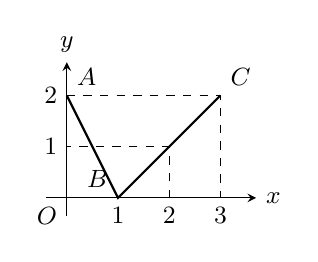
\begin{tikzpicture}[x=.65cm,y=.65cm,>=stealth,font=\small]
\draw[->](-.4,0)--(3.7,0)node[right]{$x$};\draw[->](0,-.35)--(0,2.65)node[above]{$y$};
\draw[thick](0,2)node[above right]{$A$}--(1,0)node[above left]{$B$}--(3,2)node[above right]{$C$};
\draw[dashed](0,2)--(3,2)--(3,0);\draw[dashed](2,0)--(2,1)--(0,1);
\node[below left]at(0,0){$O$};\foreach \x in {1,2,3}\node[below]at(\x,0){$\x$};
\foreach \y in {1,2}\node[left]at(0,\y){$\y$};\end{tikzpicture}\end{center}}
\renewcommand{\arraystretch}{1.2}

\newcommand{\PaperName}{D卷参考答案与评分}
\begin{document}
\begin{center}{\Large\bfseries 高一数学期中教材改编练习卷（D）}\\[2mm]参考答案、评分细则与教材出处\end{center}
单选、填空每题5分；多选全对6分，部分选对且无错项3分，含错项或未选0分。以下评分为本练习卷统一约定；解答题其他正确解法按相应步骤给分。
\parttitle{答案速查}\begin{center}\begin{tabular}{c|cccccccc}\toprule 题号&1&2&3&4&5&6&7&8\\答案&C&A&D&B&C&A&D&B\\\bottomrule\end{tabular}\par\smallskip\begin{tabular}{c|cccccc}\toprule 题号&9&10&11&12&13&14\\答案&AC&ABD&AB&$[9,+\infty)$&$1$&$[-2,2]$\\\bottomrule\end{tabular}\end{center}
\parttitle{单项选择题解析}
\ans{1}{\textbf{C}。$\complement_U B=\{0,4,5\}$，再与A取交得 $\{0,4\}$。注意补集必须在给定全集U内求。}
\ans{2}{\textbf{A}。$x>2$ 能推出 $x>0$，反向不成立，如 $x=1$。故为充分而不必要条件。}
\ans{3}{\textbf{D}。全称量词改为存在量词，范围仍为 $[-1,1]$，$\le1$ 的否定是 $>1$。}
\ans{4}{\textbf{B}。令 $t=x-2>0$，则原式为 $4+2t+8/t\ge4+2\sqrt{16}=12$；等号当且仅当 $2t=8/t$，即 $t=2,x=4$ 时成立。}
\ans{5}{\textbf{C}。A在负数处对应关系不同；B第二个函数在0无定义；C两者定义域均为 $\R$，且 $\sqrt[3]{x^9}=x^3$；D定义域分别为 $[0,+\infty)$、$(-\infty,0]$，不同。}
\ans{6}{\textbf{A}。根式要求 $x\le2$，分母要求 $x\ne\pm1$，同时满足得 $(-\infty,-1)\cup(-1,1)\cup(1,2]$，其中2可取。}
\ans{7}{\textbf{D}。$f(-2)=f(2)=5$，$f(1)=2$，所求为3。题设可由 $f(x)=x^2+1\ (x\in\R)$ 实现。}
\ans{8}{\textbf{B}。开口向上，对称轴为 $x=-a-1$。须有 $-a-1\le1$，即 $a\ge-2$；对称轴在区间左端点时仍满足严格递增。}
\parttitle{多项选择题与填空题解析}
\ans{9}{\textbf{AC}。A：乘负数c反向，正确。B：同减c应保序，错误。C：除以负数c反向，正确。D：不能由 $a<b$ 推出平方的固定次序，例如 $a=1,b=2$ 时D不成立。}
\ans{10}{\textbf{ABD}。顶点1在区间中，最大值为4；端点值 $f(-1)=0,f(2)=3$，最小值为0。函数在 $[-1,1]$ 上递增，在 $[1,2]$ 上递减；两段值域分别为 $[0,4]$、$[3,4]$，取并得 $[0,4]$。}
\ans{11}{\textbf{AB}。A：$f(-3)=f(3)<f(1)=f(-1)$；B由偶性成立。C中实际为 $f(-1)=f(1)>f(2)$，故错误。D中 $f(0)>f(1)$，故错误。}
\ans{12}{\textbf{$[9,+\infty)$}。配方得 $(x-3)^2+k-9$，最小值为 $k-9$，故充要条件为 $k\ge9$，端点9可取。}
\ans{13}{\textbf{$1$}。令 $x=1$，得到 $f(3)=2\times1-1=1$；也可令 $t=x+2$，得 $f(t)=2t-5$ 后代入。}
\ans{14}{\textbf{$[-2,2]$}。当 $x\le1$ 时 $f(x)=-2$；当 $1<x<3$ 时 $f(x)=2x-4$，值域为 $(-2,2)$；当 $x\ge3$ 时 $f(x)=2$。取并集为 $[-2,2]$。}

\newpage
\parttitle{解答题解析与分步评分}
\ans{15}{（15分）\subq{1}{$A\cap B=(1,3]$（3分），$A\cup B=[-1,5]$（3分），$\complement_U A=(-\infty,-1)\cup(3,+\infty)$（3分）。}\subq{2}{若 $t<-1$，B含有小于 $-1$ 的元素；若 $t>3$，区间 $(3,t]$ 未被覆盖，均不满足。因此必须有 $-1\le t\le3$（3分）。反之，当 $-1\le t\le3$ 时，两集合不遗漏连接点且不超出目标区间，确有 $A\cup B=[-1,5]$。故 $t\in[-1,3]$（3分）。}}
\src{p.13，习题1.1第9题；p.13，习题1.1第16题}
\ans{16}{（15分）\subq{1}{原式等价于 $(2x+3)(x-1)<0$（3分），故解集为 $(-3/2,1)$（3分）。}\subq{2}{原式等价于 $(x-m)(x+2)\le0$（3分）。当 $m<-2$ 时，解集为 $[m,-2]$（2分）；当 $m=-2$ 时，解集为 $\{-2\}$（2分）；当 $m>-2$ 时，解集为 $[-2,m]$（2分）。}}
\src{p.59，习题2.3第4题；p.59，习题2.3第8题}
\ans{17}{（17分）\subq{1}{定义域 $[-3,3]$ 关于原点对称（1分），$f(-x)=g(-x)+g(x)=f(x)$（2分），故f为偶函数（1分）。}\subq{2}{当 $x\in[-3,0)$ 时，$-x\in(0,3]$（1分），$f(-x)=x^2+2x+3$（2分），由偶性得 $f(x)=x^2+2x+3$（2分）。}\subq{3}{任取 $1\le x_1<x_2\le3$（1分），$f(x_2)-f(x_1)=(x_2-x_1)(x_1+x_2-2)>0$（2分），故在 $[1,3]$ 上严格递增（1分）。在 $[0,3]$ 上 $f(x)=(x-1)^2+2$，结合偶性，最小值为2，在 $x=\pm1$ 时取得（2分）；最大值为6，在 $x=\pm3$ 时取得（2分）。}}
\src{p.84，例5；p.90，复习题第7题；p.81，例1}
\ans{18}{（17分）\subq{1}{$64^{2/3}=16$（2分），$16^{-1/2}=1/4$，原式为 $63/4$（2分）。}\subq{2}{由 $9^\alpha=1/3=9^{-1/2}$ 得 $\alpha=-1/2$（2分），故 $f(x)=1/\sqrt x$（1分），定义域为 $(0,+\infty)$（2分）。}\subq{3}{定义域不关于原点对称，既不是奇函数也不是偶函数（2分）；单调递减区间为 $(0,+\infty)$（2分）。任取 $0<x_1<x_2$（1分），有 $f(x_1)-f(x_2)=\dfrac{\sqrt{x_2}-\sqrt{x_1}}{\sqrt{x_1}\sqrt{x_2}}>0$（2分），故函数在定义域上严格递减（1分）。}}
\src{p.104，习题4.1第4题；p.104，习题4.1第8题}
\ans{19}{（13分）\subq{1}{由 $a^2=4$ 且 $a>0$ 得 $a=2$（2分），故 $h(x)=2^x-2\ (x\in\R)$（1分）。}\subq{2}{底数大于1，$2^x$ 在 $\R$ 上严格递增，减去常数不改变单调性，故h递增（2分）。由 $2^x$ 取遍 $(0,+\infty)$，得h值域为 $(-2,+\infty)$（2分）。由 $2^x-2=0$ 得唯一零点为 $x=1$（2分）。}\subq{3}{原不等式等价于 $2^x\le8=2^3$（2分），底数大于1，故解集为 $(-\infty,3]$（2分）。}}
\src{p.112，例5；p.114，习题4.2第8题}

\newpage
\parttitle{命题结构与教材改编记录}
本卷只使用教材第1至3章及第4章4.1至4.2的例题、习题和练习作为母题。集合与逻辑30分，不等式31分，函数概念与性质59分，幂函数与指数函数30分；合计150分。
\par 主考点归类：集合1、15题共20分，逻辑2、3题共10分；基本不等式4题5分、不等式性质9题6分、恒成立12题5分、二次不等式16题15分；函数概念5、6、13题共15分，函数性质7、8、10、11、14、17题共44分；幂函数18题17分、指数函数19题13分。综合题允许知识交叉，归类用于统计，不将同一分数重复计入。
\par 教材页码指印刷页，正文PDF页序为印刷页加7。下列ID均可在教材题库中检索，改编题的答案已另行重算，不能直接套用母题答案。
\par 未特别注明的改编均为更换数据与设问、保留教材母题的概念结构。逐题目标、预期方法、易错点及评价方式另见随附“命题细目与教材出处.csv”。
\small\begin{longtable}{@{}p{.045\linewidth}p{.925\linewidth}@{}}\toprule 题号&教材母题与改编说明\\\midrule\endhead
1 & p.13，习题1.1第9题（PDF第20页）\newline{\scriptsize\ttfamily\detokenize{XJ-B1-C01-HW-P013-Y0433}}\\[3pt]
2 & p.18，例5（PDF第25页）\newline{\scriptsize\ttfamily\detokenize{XJ-B1-C01-EX-P018-Y0491}}\\[3pt]
3 & p.23，页首练习（PDF第30页）\newline{\scriptsize\ttfamily\detokenize{XJ-B1-C01-PR-P023-Y0176}}\\[3pt]
4 & p.40，练习第3题（PDF第47页）\newline{\scriptsize\ttfamily\detokenize{XJ-B1-C02-PR-P040-Y0406}}\\[3pt]
5 & p.66，例2（PDF第73页）\newline{\scriptsize\ttfamily\detokenize{XJ-B1-C03-EX-P066-Y1436}}\\[3pt]
6 & p.77，习题3.1第4题（PDF第84页）\newline{\scriptsize\ttfamily\detokenize{XJ-B1-C03-HW-P077-Y0286}}\\[3pt]
7 & p.86，习题3.2第7题（PDF第93页）\newline{\scriptsize\ttfamily\detokenize{XJ-B1-C03-HW-P086-Y0288}}\\[3pt]
8 & p.82，例3（PDF第89页）\newline{\scriptsize\ttfamily\detokenize{XJ-B1-C03-EX-P082-Y0618}}\\[3pt]
9 & p.37，练习第1题（PDF第44页）\newline{\scriptsize\ttfamily\detokenize{XJ-B1-C02-PR-P037-Y0875}}\\[3pt]
10 & p.90，复习题第7题（PDF第97页）\newline{\scriptsize\ttfamily\detokenize{XJ-B1-C03-RV-P090-Y1256}}\\[3pt]
11 & p.86，习题3.2第11题（PDF第93页）\newline{\scriptsize\ttfamily\detokenize{XJ-B1-C03-HW-P086-Y1034}}\\[3pt]
12 & p.55，例5（PDF第62页）\newline{\scriptsize\ttfamily\detokenize{XJ-B1-C02-EX-P055-Y0177}}\\[3pt]
13 & p.90，复习题第3题（PDF第97页）\newline{\scriptsize\ttfamily\detokenize{XJ-B1-C03-RV-P090-Y0678}}\\[3pt]
14 & p.76，练习第1题（PDF第83页）\newline{\scriptsize\ttfamily\detokenize{XJ-B1-C03-PR-P076-Y0217}}\\[3pt]
15 & p.13，习题1.1第9题（PDF第20页）；p.13，习题1.1第16题（PDF第20页）\newline{\scriptsize\ttfamily\detokenize{XJ-B1-C01-HW-P013-Y0433 / XJ-B1-C01-HW-P013-Y1442}}\newline 改编：更换为有界区间的交并补运算，增加并集恰好等于指定区间时的参数上下界判断。\\[3pt]
16 & p.59，习题2.3第4题（PDF第66页）；p.59，习题2.3第8题（PDF第66页）\newline{\scriptsize\ttfamily\detokenize{XJ-B1-C02-HW-P059-Y0221 / XJ-B1-C02-HW-P059-Y0874}}\\[3pt]
17 & p.84，例5（PDF第91页）；p.90，复习题第7题（PDF第97页）；p.81，例1（PDF第88页）\newline{\scriptsize\ttfamily\detokenize{XJ-B1-C03-EX-P084-Y0592 / XJ-B1-C03-RV-P090-Y1256 / XJ-B1-C03-EX-P081-Y0375}}\newline 改编：融合偶对称构造、区间最值和作差证明，修改正半轴表达式并要求列出全部对称最值点。\\[3pt]
18 & p.104，习题4.1第4题（PDF第111页）；p.104，习题4.1第8题（PDF第111页）\newline{\scriptsize\ttfamily\detokenize{XJ-B1-C04-HW-P104-Y0874 / XJ-B1-C04-HW-P104-Y1494}}\\[3pt]
19 & p.112，例5（PDF第119页）；p.114，习题4.2第8题（PDF第121页）\newline{\scriptsize\ttfamily\detokenize{XJ-B1-C04-EX-P112-Y0737 / XJ-B1-C04-HW-P114-Y0667}}\newline 改编：由教材指数函数定底数和纵向平移母题改编，改为底数大于1，考查平移后的值域、零点与不等式。\\[3pt]
\bottomrule\end{longtable}\normalsize
\par\textbf{评价与复习建议：}客观题逐项判断，填空题核对端点和可取性；解答题按列式、推理、分类完整性及结论评分。第17、18题重点观察能否从定义出发说明理由。上述难度与错误仅为教学预判，未经过班级试测，不预设均分或达标率。
\end{document}
